\documentclass[letterpaper]{article}
\usepackage[submission]{aaai2027}
\usepackage[hyphens]{url}
\usepackage{graphicx}
\urlstyle{rm}
\def\UrlFont{\rm}
\usepackage{natbib}
\usepackage{caption}
\frenchspacing
\usepackage{booktabs}
\usepackage{array}
\usepackage{placeins}

\pdfinfo{
/TemplateVersion (2027.1)
}

\setcounter{secnumdepth}{0}

\title{When Is Decision-Focused Learning Useful for Graph Combinatorial Optimization?}
\author{Anonymous Submission}
\affiliations{}

\begin{document}

\maketitle

\begin{abstract}
Decision-focused learning can substantially improve predict-then-optimize
pipelines when prediction errors change the value of the downstream decision.
However, in some graph combinatorial optimization problems, different feasible
solutions may be close substitutes under the true objective. We study this
phenomenon in kidney exchange and contrast it with shortest-path benchmarks.
Our working hypothesis is that the benefit of decision-focused learning depends
not only on whether prediction errors change the selected solution, but on
whether the alternative solution is materially worse. We combine direct
code-path validation, decision-level error analysis, randomized toy
experiments, and KEP sensitivity analyses to show that solution identity can
change frequently while regret remains small when close substitutes exist,
whereas larger oracle--second-best gaps create more room for
decision-focused learning.
\end{abstract}

\section{Introduction}

Predict-then-optimize pipelines are often evaluated by prediction error even
though the final objective is decision quality. Decision-focused learning (DFL)
addresses this mismatch by training predictors through an optimization-aware
surrogate such as SPO+ \citep{elmachtoub2022smart}. In shortest-path benchmarks,
this idea can produce large gains over a two-stage mean-squared-error baseline.
In our kidney-exchange experiments, however, the gains are more modest.

This paper asks a targeted question: when is DFL useful for graph combinatorial
optimization? Our starting point is that selected-solution identity is not
enough. A model can select a different feasible solution from the oracle and
still achieve nearly the same objective value. This can happen in decomposable
packing-style problems, where many feasible solutions are assembled from mostly
independent components and close substitutes are common.

We therefore analyze prediction errors at the decision level. Rather than asking
only which edge weights are predicted poorly, we ask whether the badly predicted
edges participate in the symmetric difference between selected and oracle
solutions, and whether the alternative solution is truly worse.

\paragraph{Contributions.}
We make three contributions. First, we validate the relevant SPO+ training path
against independent reference implementations so that later interpretation is
not confounded by implementation bugs. Second, we provide decision-level
diagnostics for kidney exchange that distinguish decision-critical prediction
errors from irrelevant prediction errors. Third, we build a toy family showing
that close-substitute behavior is not specific to one hand-picked instance: it
appears across several packing-style structures and contrasts with path-like
negative controls.

\section{Problem Setup}

We study graph optimization problems with uncertain objective coefficients. Each
instance has features $x$, true coefficients $c$, and a feasible set
$\mathcal{Y}(x)$. A predictor outputs $\hat{c}$, and the downstream decision is
obtained by solving
\[
    \hat{y} \in \arg\max_{y \in \mathcal{Y}(x)} \hat{c}^{\top}y
\]
for reward-maximization problems, with the analogous minimization form for
shortest path.

The two-stage baseline trains $\hat{c}$ to minimize prediction error. DFL
methods instead use a surrogate for downstream regret or decision loss. For
SPO+, the reward-maximization form used in our implementation compares the
oracle solution $y^\star$ with an adversarial solution under shifted costs
$2\hat{c}-c$.

We report normalized decision gap relative to the oracle objective. We also use
solution-overlap diagnostics, including whether the selected solution matches
the oracle and the edge Jaccard similarity between selected and oracle
solutions.

\section{Mechanism: Close Substitutes}

Our central hypothesis is that DFL is most useful when prediction errors change
the objective value of the selected solution, not merely its identity. In
packing-style graph problems, feasible solutions can be composed of several
components. If each component has close substitutes, a prediction error may swap
one feasible solution for another while changing the true objective only
slightly.

This mechanism predicts two empirical patterns. First, solution identity can
change even when normalized regret remains small. Second, all-edge prediction
error should be a weak explanation of decision gap compared with error on
decision-changing edges, such as edges in the symmetric difference between the
oracle and selected solutions.

This framing avoids a stronger claim that DFL is unnecessary for all packing
problems. The claim is conditional: when the feasible landscape contains many
near-optimal alternatives, DFL has less room to improve over a strong two-stage
model; when prediction errors redirect a coupled decision to a much worse
solution, DFL can matter substantially.

\section{Toy Examples}

Figure~\ref{fig:toy-regret} summarizes the expanded toy family. In the
packing-style examples, two-stage prediction changes the selected solution but
the normalized gap remains below the 5\% reference line. In the path-like
controls, a ranking error redirects the whole connected path and creates much
larger regret.

\begin{figure}[t]
    \centering
    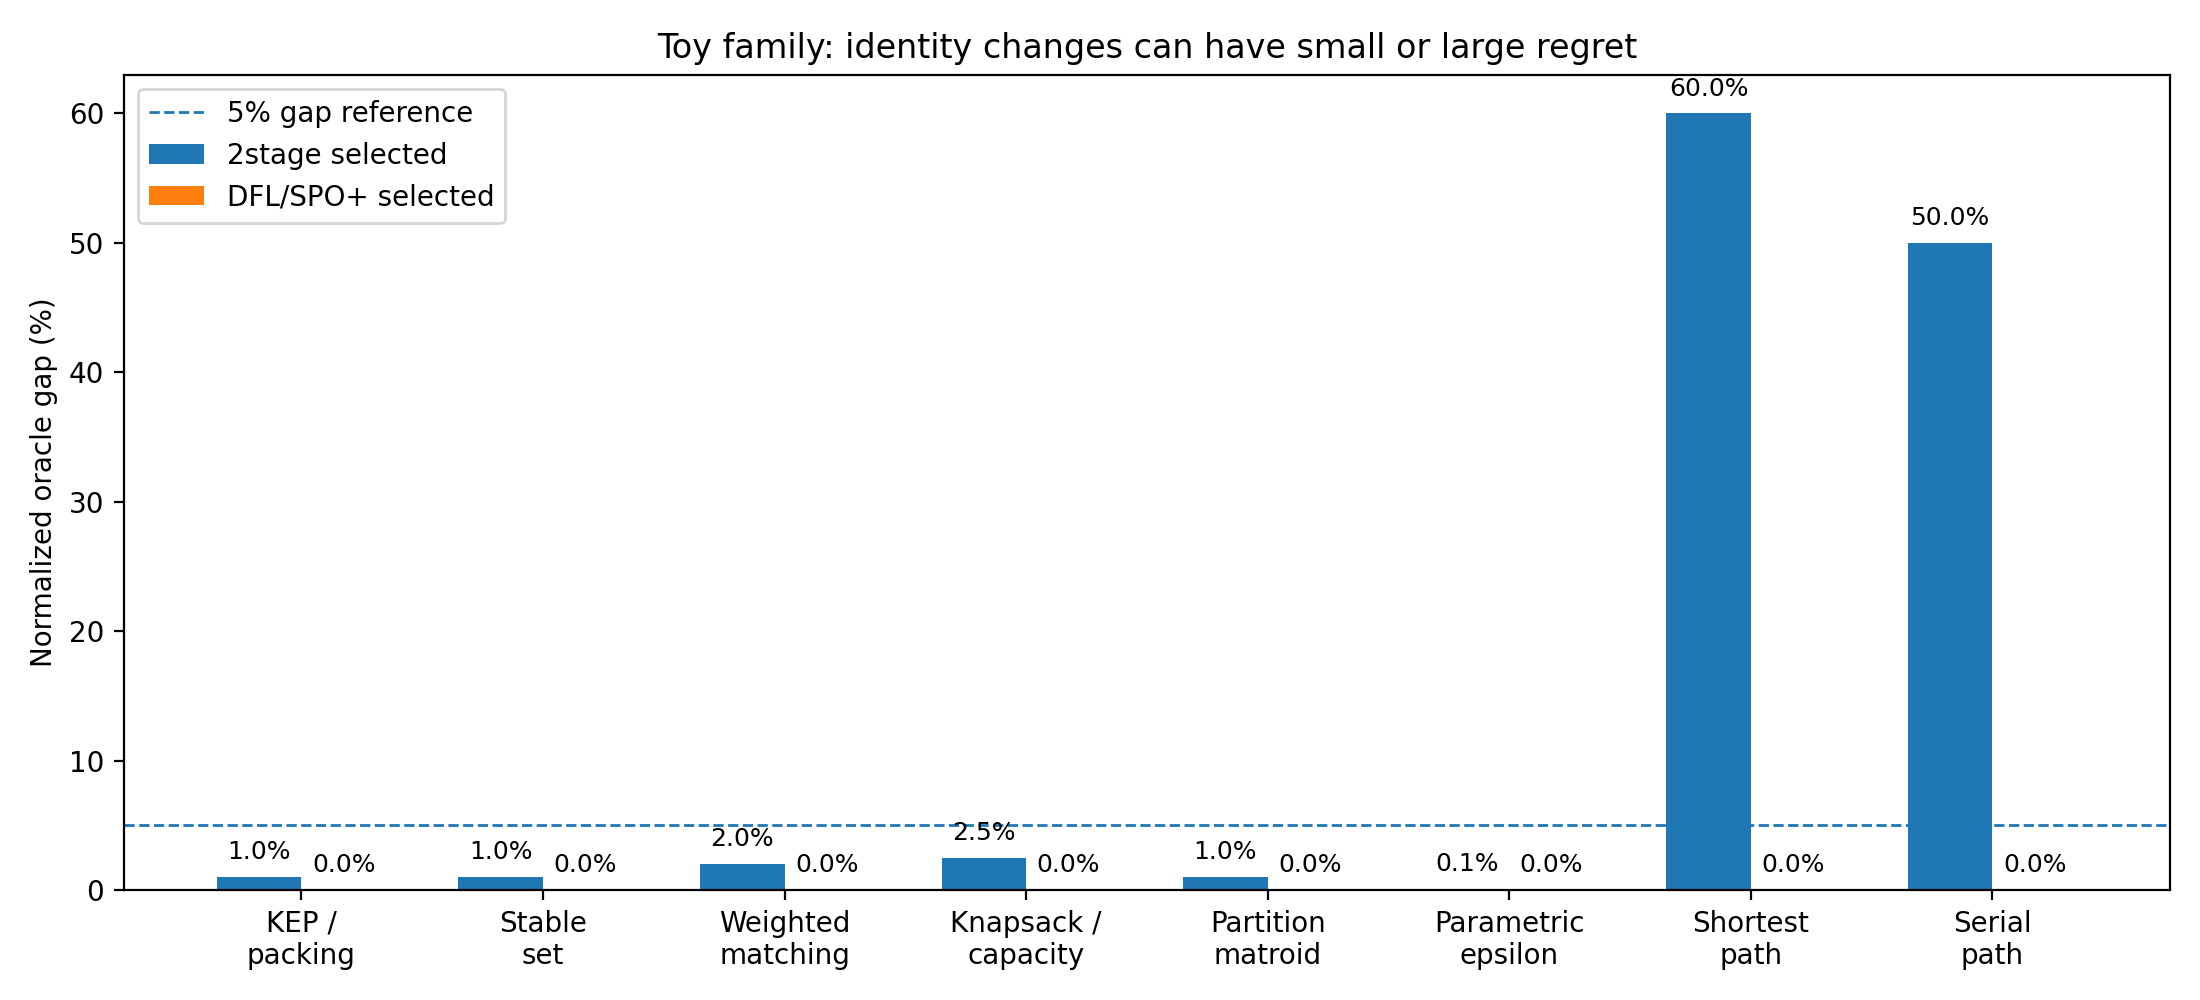
\includegraphics[width=\linewidth]{figures/toy_regret_comparison.png}
    \caption{Toy family showing that solution identity changes can correspond
    to either small or large regret. Packing-style positive examples have close
    substitutes; path-like negative controls do not.}
    \label{fig:toy-regret}
\end{figure}

\begin{figure}[t]
    \centering
    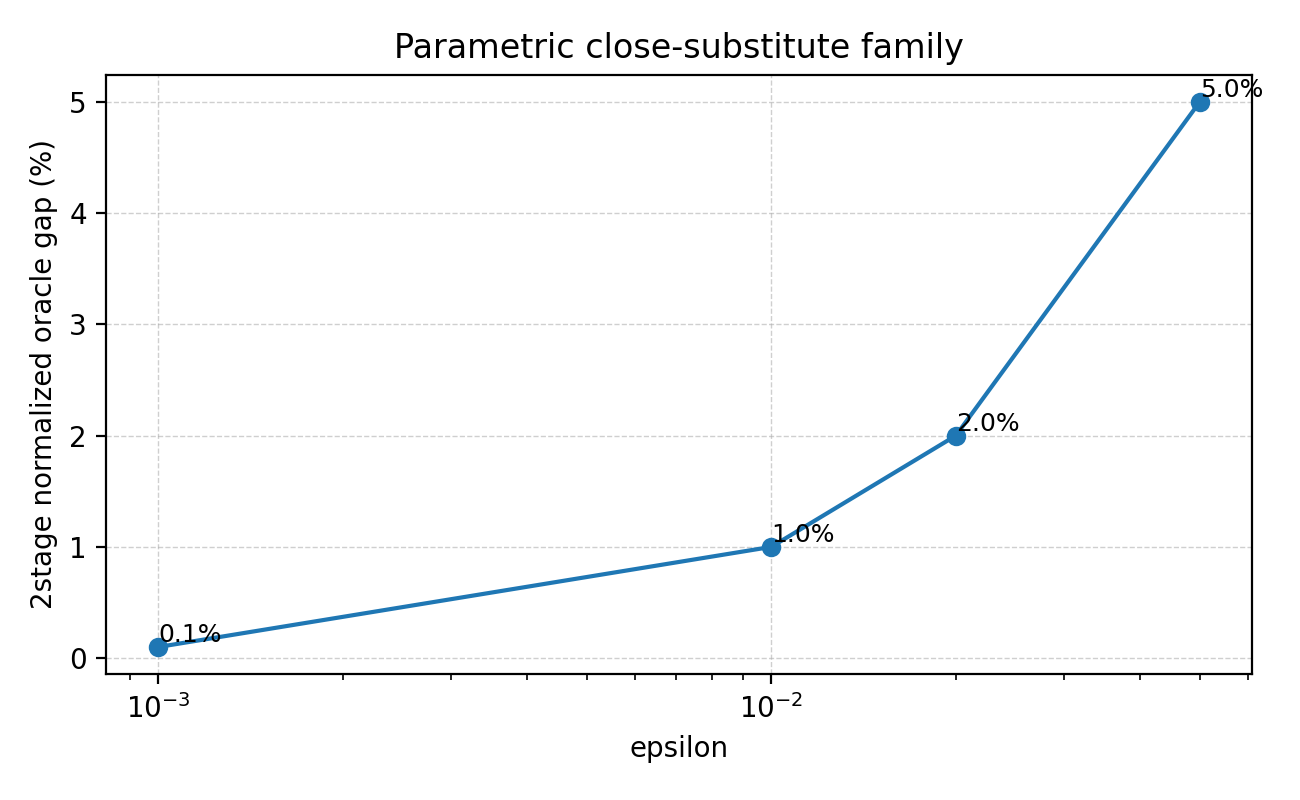
\includegraphics[width=\linewidth]{figures/toy_parametric_epsilon_curve.png}
    \caption{Parametric close-substitute construction. The selected solution
    changes for every $\epsilon$, but the normalized regret is exactly
    $\epsilon$ and can be made arbitrarily small.}
    \label{fig:toy-epsilon}
\end{figure}

Table~\ref{tab:toy-summary} lists the oracle and two-stage selected solutions
for each toy problem family.

\begin{table*}[t]
    \centering
    \caption{Toy examples for the close-substitute mechanism and path-like
    negative controls.}
    \label{tab:toy-summary}
    \small
    \setlength{\tabcolsep}{3pt}
    \begin{tabular}{llll}
\toprule
Problem & Oracle / true best & 2stage selected & 2stage normalized gap \\
\midrule
KEP / set packing & C12 + C34, value 20 & C13 + C24, value 19.8 & 1.0\% \\
Stable set & A + B, value 20 & C + D, value 19.8 & 1.0\% \\
Weighted matching & M12 + M34, value 20 & M13 + M24, value 19.6 & 2.0\% \\
Cardinality knapsack & A + B, value 20 & C + D, value 19.5 & 2.5\% \\
Partition matroid & A1 + B1, value 20 & A2 + B2, value 19.8 & 1.0\% \\
Parametric packing family & S\_star, value 1 & S\_epsilon, value 0.999 & 0.1\% \\
Shortest path & Path A: s-a1-a2-t, cost 5 & Path B: s-b1-b2-t, cost 8 & 60.0\% \\
Serial path control & Serial route A: low-cost chain, cost 10 & Serial route B: high-cost chain, cost 15 & 50.0\% \\
\bottomrule
\end{tabular}

\end{table*}

The parametric construction is the most direct generality argument. It contains
two complete feasible solutions, $S_\star$ and $S_\epsilon$, with true values
$1$ and $1-\epsilon$. If the two-stage predictor slightly overestimates
$S_\epsilon$, it selects the wrong solution identity. Nevertheless, normalized
regret is only $\epsilon$.

\section{Experiments and Diagnostics}

The empirical analysis focuses on kidney-exchange prediction tasks and
shortest-path controls. For kidney exchange, we compare a two-stage predictor
selected by validation MSE with SPO+ models selected by validation decision
metrics. We evaluate on held-out graph instances and summarize normalized
decision gap, solution overlap, and edge-level prediction-error diagnostics.

The current decision-analysis evidence supports the close-substitute story in
two ways. First, many different selected solutions are near ties under the true
objective. Second, raw all-edge MSE is much less aligned with decision gap than
error concentrated on decision-changing edges. This suggests that prediction
errors matter most when they alter the selected feasible components in a way
that harms the true objective.

The final paper should report the main decision-analysis tables and plots here:
case-study summaries, observed-candidate near-tie statistics, and
decision-critical MSE correlations.

\section{Discussion}

\paragraph{Guideline.}
The main takeaway is not that DFL is broadly unnecessary, but that its room for
improvement depends on how prediction errors affect the downstream objective.
DFL is most useful when prediction errors change the objective value of the
selected solution, not merely its identity. If a predictor selects a different
feasible solution whose true value is nearly oracle-level, then the normalized
regret left for any decision-aware training method to remove is small.

\paragraph{When two-stage may be enough.}
In problems with close substitute solutions, a two-stage model can have decision
performance similar to DFL even when it does not recover the oracle solution
identity. This is especially plausible in decomposable packing-style feasible
sets, where a solution is assembled from multiple components and one component
can often be exchanged for another with little loss in objective value. Our KEP
rank-2 evidence, cycle-length sensitivity, density perturbations, and case
studies all point to this mechanism: many alternative packings remain close to
the oracle under the true objective.

\paragraph{When DFL may help.}
The contrast is that some feasible sets amplify local prediction errors. In
coupled or path-like problems, an incorrect local preference can redirect the
whole decision rather than swapping one nearly equivalent component. In that
setting, selected-solution identity and objective value are more tightly linked,
and DFL can have substantially more room to improve over a two-stage baseline.
This helps explain why shortest-path benchmarks can show large SPO+ gains while
KEP-like packing problems may show more similar performance between two-stage
and optimization-aware training.

\paragraph{Limitations.}
Our KEP experiments cover one synthetic regime, so the numerical magnitudes
should not be read as universal constants for kidney exchange. The density
sensitivity analysis uses selected case graphs rather than a full distributional
benchmark, and the randomized toy experiments are controlled mechanism studies
rather than full benchmark evidence. They also clarify that the claim is
conditional: packing and stable-set problems are not automatically easy for
two-stage models. When prediction noise selects many wrong local components, or
when alternatives are well separated, regret can increase and DFL has more room
to help. The evidence supports the proposed explanation, but broader benchmarks
are needed before treating Property X as a complete taxonomy of when DFL helps.

\paragraph{Future work.}
A natural next step is to test Property X directly on standard stable-set, set
packing, matching, and knapsack-style benchmarks. The key empirical question is
whether best/second-best diagnostics can predict when two-stage and DFL methods
will have similar decision performance. If this diagnostic transfers across
problem classes, it could become a practical pre-check for whether the extra
complexity of decision-focused training is likely to pay off.


\bibliography{references}

\end{document}
